\documentclass[11pt]{article}
\usepackage[margin=1in]{geometry}
\usepackage{graphicx}
\usepackage{booktabs}
\usepackage{hyperref}
\hypersetup{colorlinks=true,linkcolor=blue,urlcolor=blue}
\title{Episode-Start Label Dataset Report}
\author{TP2 SPY Call Pipeline}
\date{June 2026}
\begin{document}
\maketitle

\section*{Purpose}
This report documents the episode-start label dataset. Each row represents the
first day of a TP2 pair episode, joined to point-in-time detector features and
future outcome labels. Only \texttt{feature\_*} columns are eligible for ML
inputs. Future outcome columns are retained only as labels or diagnostics.

\section*{Validation}
\begin{center}
\begin{tabular}{lr}
\toprule
Metric & Value \\
\midrule
Episode-start label rows & 2,098,213 \\
Unique episode IDs & 2,098,213 \\
Duplicate episode IDs & 0 \\
Missing end-state labels & 0 \\
Missing start detector features & 0 \\
Observable next-state share & 52.13\% \\
True reversion share among observable rows & 97.38\% \\
\bottomrule
\end{tabular}
\end{center}

\section*{Label Mix}
\begin{figure}[h]
\centering
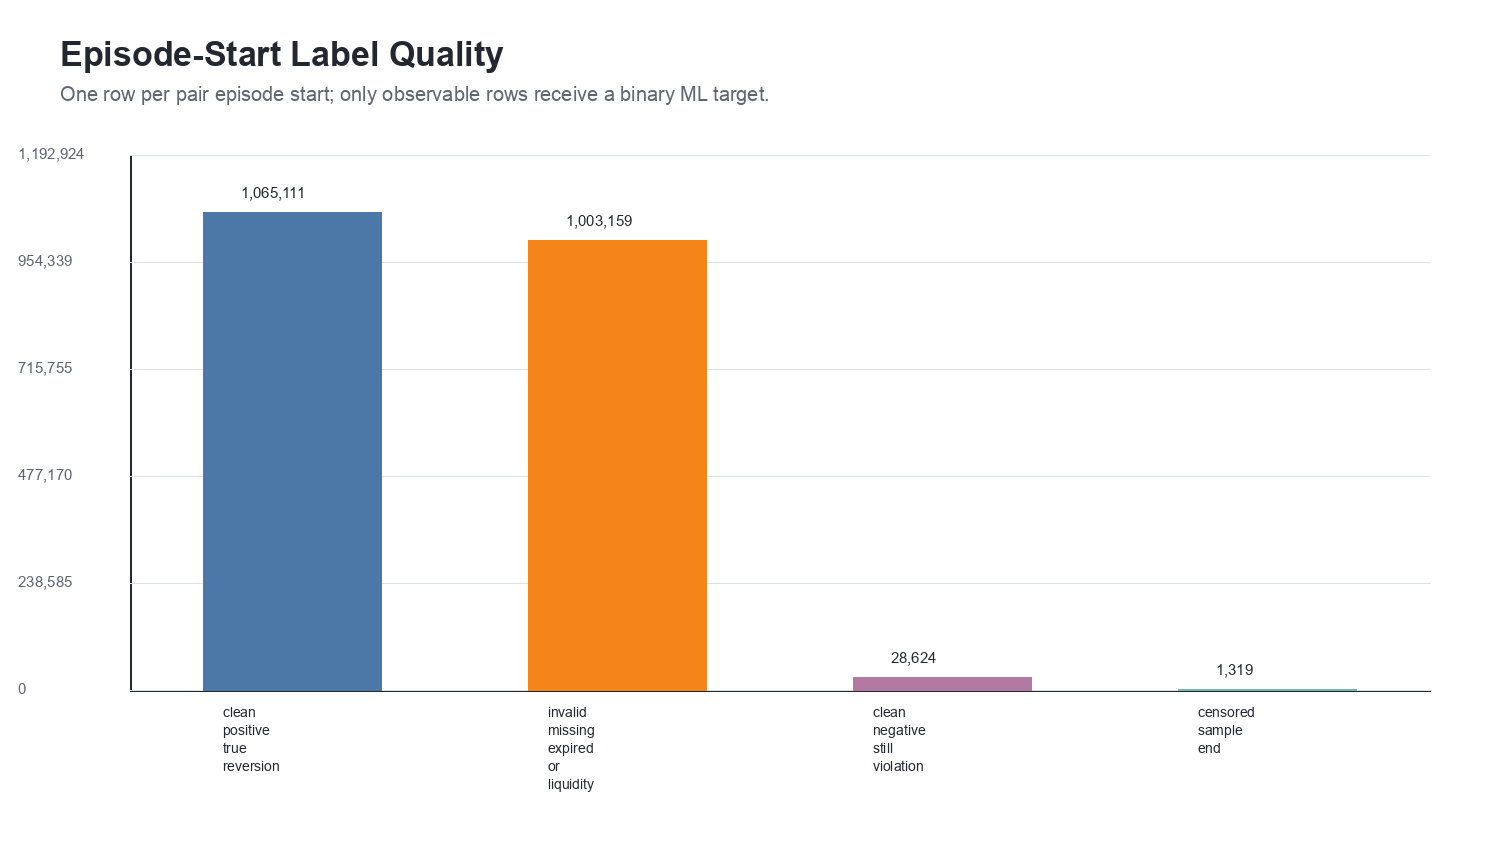
\includegraphics[width=\linewidth]{figures/episode_start_label_quality_counts.png}
\caption{Label quality counts for episode-start rows.}
\end{figure}

\begin{figure}[h]
\centering
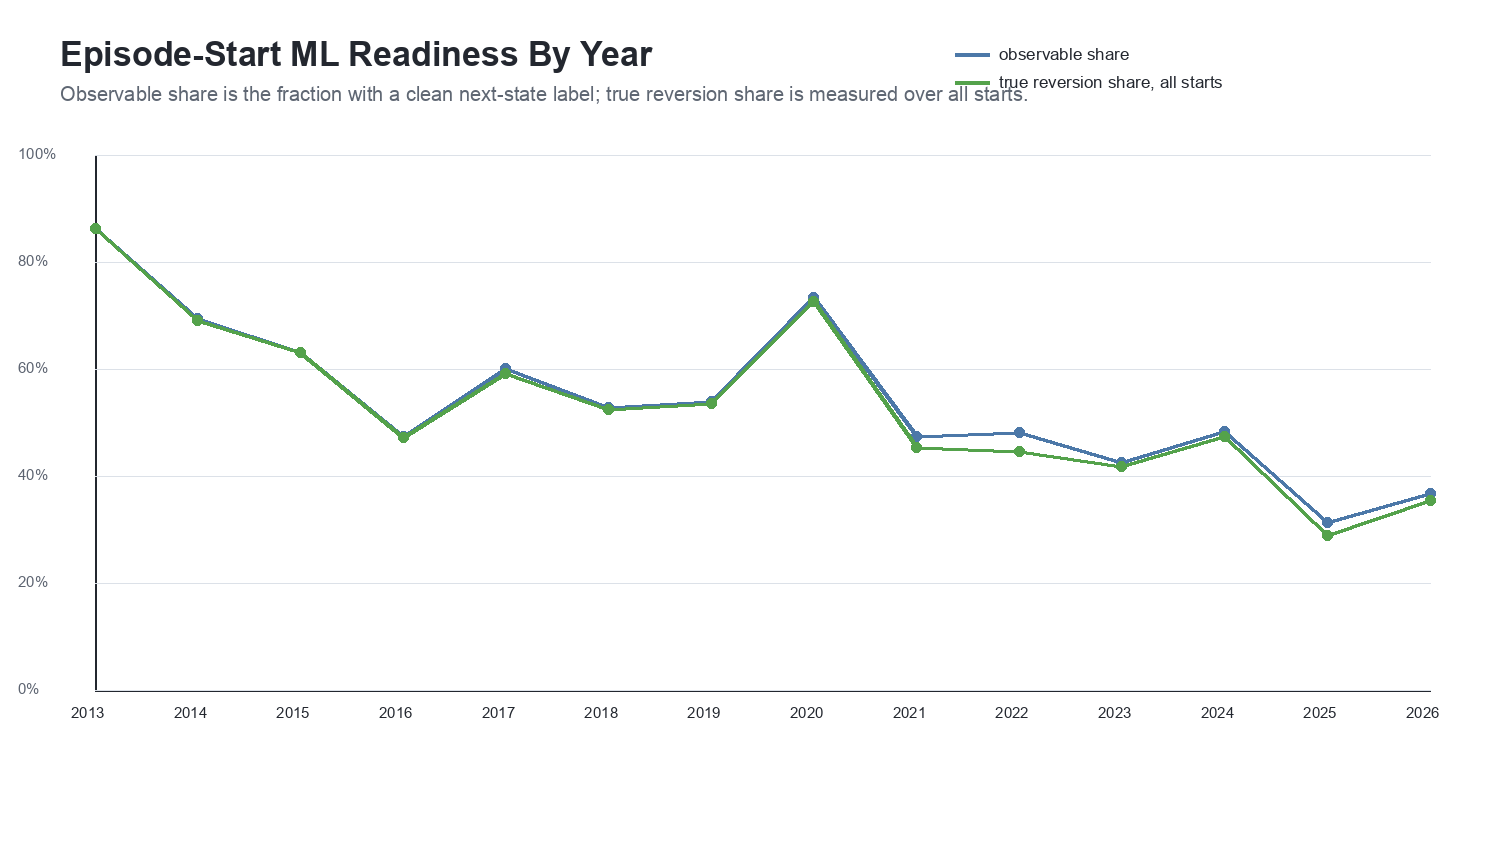
\includegraphics[width=\linewidth]{figures/episode_start_ml_readiness_by_year.png}
\caption{Observable and true-reversion shares by signal year.}
\end{figure}

\section*{Leakage Rule}
The model may use only information known at the signal date: detector geometry,
entry liquidity, moneyness, spread, volume/open-interest, and prior lifecycle
features. It must not use episode end date, future reversion status, realized
P\&L, exit availability, or any \texttt{label\_*} column.

\end{document}
